% !TEX root = Thesis.tex

%==============================================================================
\chapter{Results and discussion}
\label{chap:results_and_discussion}
%==============================================================================

Once the theoretical description of the experiment has been completely introduced, the following part consist in the exposition of the obtained results together with a discussion concerning its correspondence with the announced theory. Due to this, the first step must be the Raman beams characterization with the measurement of each beam radius. This will allow in the next parts to make a direct correlation between beam power and intensity, which will be crucial for the whole experiment characterization.

\section{Measurement of the Raman beams radius}

These laser beams of the \SI{841}{\nano\meter} transition have been considered during all the theory as Gaussian beams. Therefore, they are described spatially by Equation \eqref{eq:intensity_gaussian}, which gives the relation between beam power $P$ and maximum intensity $I_{0}$ as
\begin{equation}
	I_0 = \frac{2P}{\pi w_0^2}
\end{equation}

Where $w_0$ represents the beam radius at the atomic cloud position. Thus, a measurement of this quantity must be performed in order to obtain $I_0$ from the beam power. Figure \ref{fig:raman_beams_radius} shows both horizontal and vertical measurements for the two beams with the use of a knife-edge method. These data points were fit to an error function, which gave the estimations for $w_0$ in every case. From averaging the vertical and horizontal estimations of $w_0$ one gets the final measurement to be
\begin{align*}
	w_{01} &= (0.4961\pm0.0012)\si{\milli\meter}   &   w_{02} &= (0.8778\pm0.0024)\si{\milli\meter}
\end{align*}

Note that the use of 1 and 2 for the Raman beams is also used as a distinction tool in Figure \ref{fig:raman_set_up}. As one can observe, the difference in size between both beams is approximately a factor of 3. This must be compensated by adjusting the beam powers; however, it is a strong mismatch in the parameters that could not be solved due to time constraints. Therefore, the discussion part of the following measurements will have into account this mismatch in beam sizes as a source of possible non-correspondence between theory and experiment.

\pagebreak

\begin{figure}
	\centering
	\begin{subfigure}{.5\textwidth}
		\centering
		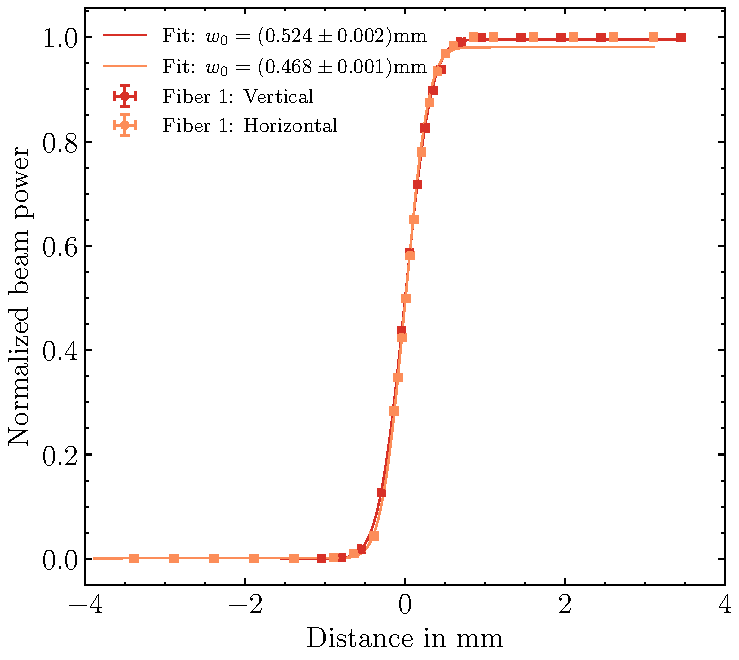
\includegraphics[width=1.\linewidth]{Fiber 1.pdf}
		\caption{Raman beam 1 (R1)}
		\label{fig:raman_beams_radius_1}
	\end{subfigure}%
	\begin{subfigure}{.5\textwidth}
		\centering
		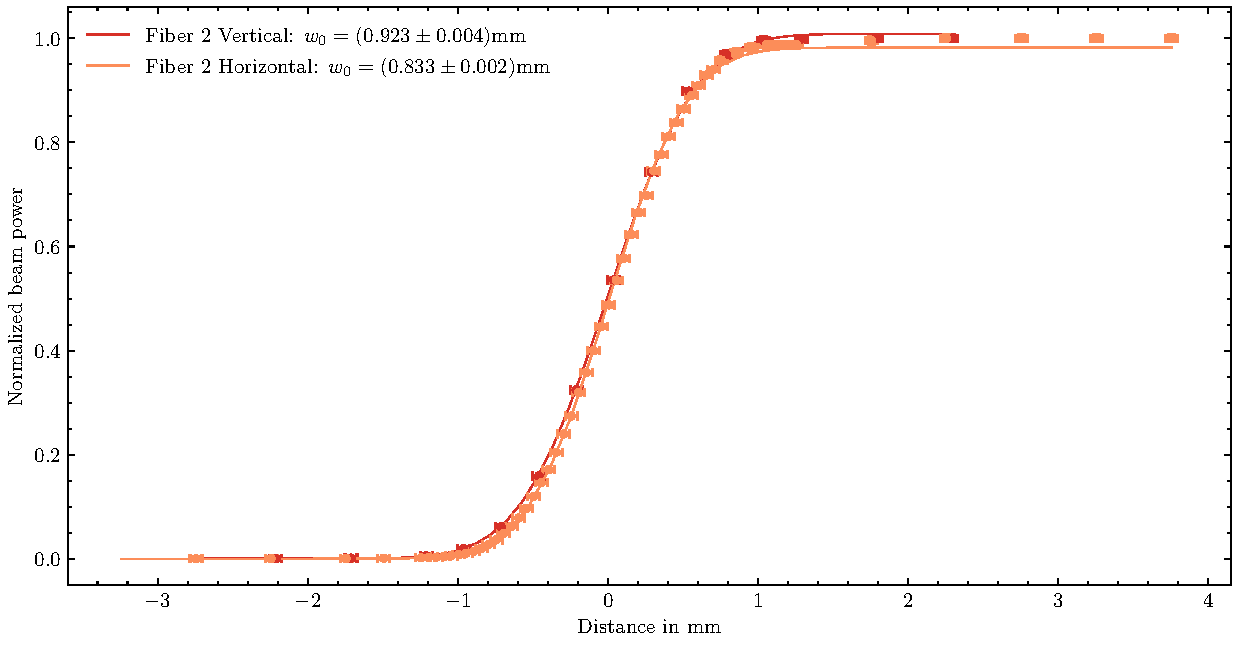
\includegraphics[width=0.955\linewidth]{Fiber 2.pdf}
		\caption{Raman beam 2 (R2)}
		\label{fig:raman_beams_radius_2}
	\end{subfigure}
	\caption[Beam radius measurement of the Raman beams performed with a knife-edge method]{Beam radius measurement of the Raman beams performed with a knife-edge method. The beam profile was measured at approximately the atomic cloud position. Each of the beams were measured in a vertical (red) and horizontal (orange) position.}
	\label{fig:raman_beams_radius}
\end{figure}


\section{Characterization of the \SI{841}{\nano\meter} erbium transition with a \ac{bec}}

The following part consists in studying the \SI{841}{\nano\meter} erbium transition by blocking arbitrarily the beam R2 and allowing R1 to interact freely with the erbium \ac{bec}. This way, the Raman beam frequency can be locked in every cycle to a specific value. After an interaction time of 10\si{\milli\second} before the final part of the evaporation phase, the atomic ensemble falls freely during a \ac{tof} of 20\si{\milli\second}. Then, the measurement is taken with the absorption imaging phase. From these measurements, the number of atoms can be estimated and the result, after scanning the frequency of R1, is shown in Figure \ref{fig:resonance_841_transition}. The maximum number of atoms measured is the normalization factor and has the value $N_\text{max} = 34849$. As it can be seen from the image, the plot shows a drop in the atom number when R1 is locked to a wavelength of approximately \SI{840.98827}{\nano\meter} in air. This is because most of the atoms forming a \ac{bec} are resonant at this wavelength get excited by the R1 beam, which expel them out of the ensemble and reduce drastically the atom number. In order to avoid effects like power broadening, the optical power of R1 has been kept as low as possible: $P_{\text{R1}} = (49.0 \pm 0.5) \si{\milli\watt}$. This way, the Gaussian fit performed in Figure \ref{fig:resonance_841_transition} gives an estimation of the resonant wavelength $\lambda_0^*$ and the linewidth broadened mostly due to the beam power $\Delta\nu_{\text{PB}}$ as
\begin{align*}
	\lambda_0^* &= 840.988266(2)\si{\nano\meter}   &   \Delta\nu_{\text{PB}} &= (3600 \pm 1700)\si{\kilo\hertz}
\end{align*}

The result is a quite accurate estimation of $\lambda_0^*$ while the calculation for $\Delta\nu_{\text{PB}}$ is not. The main reason is due to limitations in the scanning precision of the wave-meter, which was locking the laser. In any case, the measurement of $\Delta\nu_{\text{PB}}$ is helpful when comparing it to the theoretical linewidth of the transition $\Delta\nu_0 = \SI{7.96}{\kilo\hertz}$ (see Table \ref{tab:Transitions}). Giving a real scenario of how big the one-photon detuning $\delta$ must be to make reasonable the approximations used for the Raman transition processes. On the other hand, the estimation of $\lambda_0^*$ seems to be very precise, but there is a source of errors that has not been considered so far. This is the uncertainty coming from the laser frequency lock, which can not be assumed to remain constant and may shift during measurements. For this reason, the one-photon detuning $\delta$ estimation will be obtained with by using as resonance wavelength in air the following value:
\begin{equation*}
	\lambda_{0} = 840.98827(1)\si{\nano\meter}
\end{equation*}

\begin{figure}\centering
	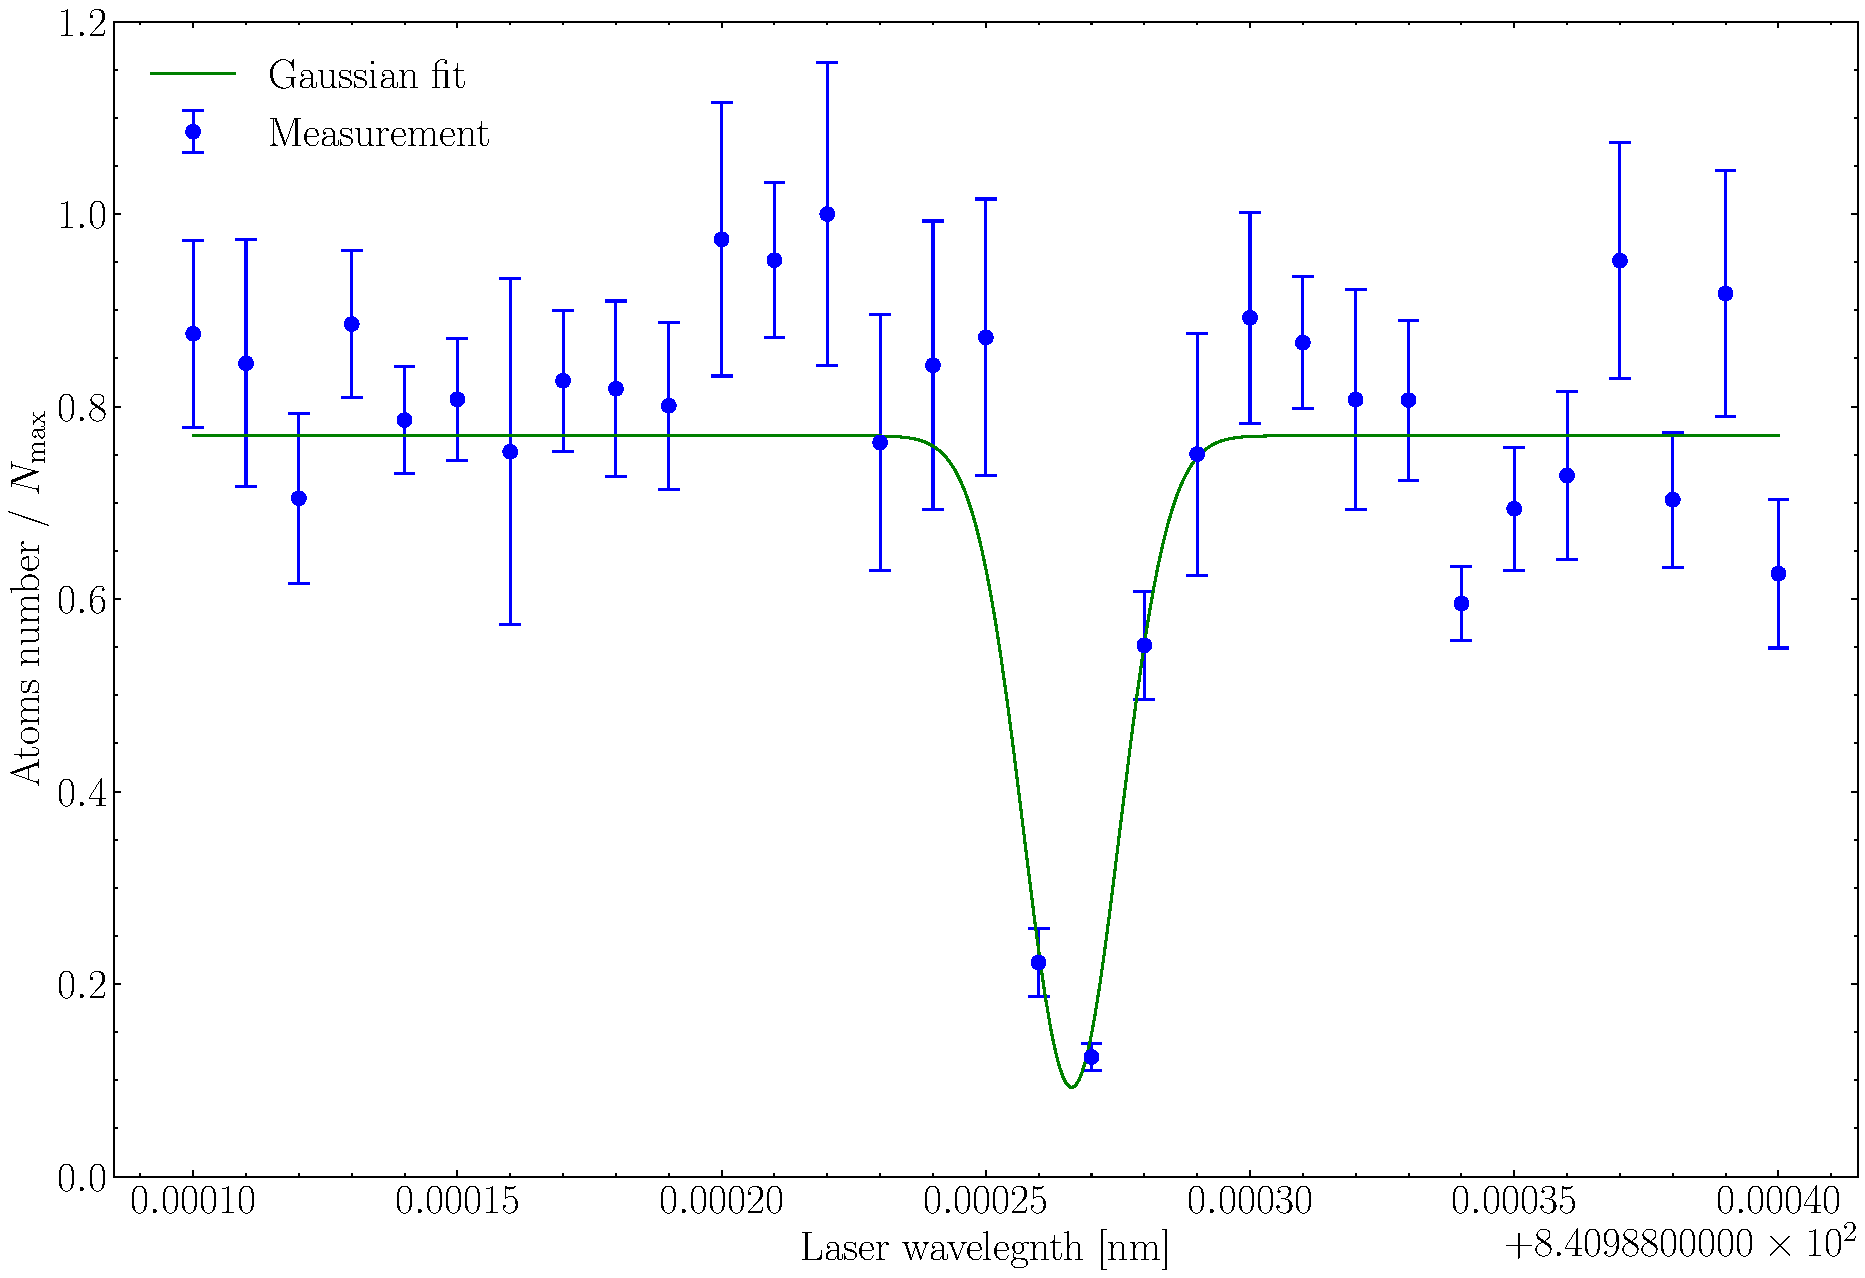
\includegraphics[width=1.\columnwidth]{Plot_resonance.pdf}
	\caption[Interaction of an erbium \ac{bec} with the beam R1]{Interaction of an erbium \ac{bec} with the beam R1. The plot shows the atom number of the \ac{bec}, normalized to the maximum measured value, as a function of the R1 wavelength in air. The interaction between R1 and the atomic ensemble lasts 10\si{\milli\second} before the end of evaporation phase in every experimental cycle. Each measured point has been obtained by averaging the atom number of 5 experimental cycles. }\label{fig:resonance_841_transition}
\end{figure}

\section{Diffraction of an erbium \ac{bec} with a 1D-lattice}

Now, it is the moment to study the diffraction of an erbium \ac{bec} with the described Raman lattice set-up. In order to do this, the one photon detuning $\delta$ must be measured. Due to the conclusions made in previous section, the optical frequency of the Raman beams has been chosen for this whole part to be $\lambda_\text{R} = 840.98880(1) \si{\nano\meter}$. Thus, the resulting value for $\delta$ turns out to be
\begin{equation*}
	\delta = 2\pi c\cdot\bigg(\frac{1}{\lambda_{0}} - \frac{1}{\lambda_\text{R}} \bigg) = 2\pi \cdot(225 \pm 6) \si{\mega\hertz}
\end{equation*}

Therefore, the approximations used for the Hamiltonian in Section \ref{subsec:diffraction_regimes} are fulfilled. Because $\delta \gg \Gamma, \Delta\nu_0$ being the decay rate $\Gamma$ and natural linewidth $\Delta\nu_0$ of the \SI{841}{\nano\meter} transition (see Table \ref{tab:Transitions}). One last approximation that has been performed is for the atomic detuning $\delta \gg \Delta_1$, with the 2-photon recoil frequency $\Delta_1$ given by Equation \eqref{eq:Bragg_condition} with $n=1$. 

\subsection{Bragg regime}

%%% Local Variables: 
%%% mode: latex
%%% TeX-master: "Thesis"
%%% End: 
